\chapter{Release 2: Gestion des équipements et Gestion des Suivis}



% Une section

% Exemple d'une section qui porte une référence à une bibliographie
% NB: il faut bien suivre le syntaxe pour ne pas tomber dans le cas où il y a une référence dans la table des matières.

\section*{Introduction}
Dans ce chapitre, nous vous présenterons les différentes étapes de la deuxième release intitulée "Gestion des équipements et gestion des suivis", qui permet de gérer la gestion des équipements et la gestion des suivis de statistiques et d'inventaire, ainsi que la "Maintenance des équipements", où nous allons gérer l'affectation des équipements aux employés et gérer les demandes de missions des équipements, ainsi que l'historique des affectations. 

Ce chapitre illustre le cycle de vie du deuxième et du troisième sprint, à savoir le backlog, la spécification fonctionnelle, la conception et la réalisation de chaque sprint.

\section{sprint 2:Gestion des équipements et Gestion des Suivis} 

Dans cette section nous allons présenter les différents étapes de la réalisation du sprint "Gestion des équipements et Gestion des Suivis".
    \subsection{Objectifs du sprint 2}
 L'objectif principal est de mettre en place les fonctionnalités nécessaires pour assurer une gestion efficace du stock d'équipements informatiques. Ces fonctionnalités comprennent l'ajout, la modification et la suppression d'équipements, quelle que soit leur catégorie (desktop, laptop, switcher, etc.). Nous cherchons également à mettre en place un système de suivi des inventaires des équipements, permettant de les classer par type.
 
 De plus, notre objectif est d'assurer le suivi des statistiques des équipements, en termes de types, d'états et de disponibilités. Cette fonctionnalité permettra aux utilisateurs d'accéder rapidement aux informations clés concernant les équipements, facilitant ainsi leur gestion et leur utilisation optimale. En atteignant ces objectifs, nous serons en mesure de fournir aux utilisateurs un système de gestion des équipements robuste et efficace, contribuant ainsi à une meilleure gestion du parc informatique de l'entreprise.

\subsection{Cycle de vie d'un équipement}

Dans le cadre de cette release, un équipement n'est pas considéré comme une simple ligne d'inventaire. Il s'agit d'un actif qui possède un cycle de vie complet. Ce cycle commence à la réception du matériel, se poursuit par l'enregistrement dans la base, la mise en stock, l'affectation à un employé ou l'utilisation dans une mission, puis se termine éventuellement par la maintenance, le retour en stock ou la sortie du parc.

Les états principaux retenus sont les suivants :

\begin{itemize}[label=\textbullet,font=\normalsize]
    \item \textbf{Disponible :} l'équipement est présent en stock et peut être affecté.
    \item \textbf{Affecté :} l'équipement est attribué à un employé pour un usage régulier.
    \item \textbf{En mission :} l'équipement est prêté temporairement pour une durée déterminée.
    \item \textbf{En maintenance :} l'équipement nécessite une intervention technique avant réutilisation.
    \item \textbf{Hors service :} l'équipement ne peut plus être utilisé et doit être remplacé ou réformé.
\end{itemize}

Cette modélisation des états facilite le suivi de disponibilité et réduit les risques de confusion entre les équipements réellement libres et ceux qui sont simplement absents du stock physique.

\subsection{Données nécessaires à la gestion des équipements}

Pour qu'un inventaire soit utile, chaque équipement doit être décrit avec des informations suffisamment précises. Les données retenues permettent d'identifier le matériel, de le localiser, de connaître son état et de retrouver son historique.

\begin{longtable}{|m{4cm}|m{6cm}|m{4cm}|}
\hline
\textbf{Donnée} & \textbf{Utilité} & \textbf{Exemple} \\
\hline
\endhead
\endfoot
\endlastfoot
\hline
Type d'équipement & Classer le matériel et calculer les statistiques & Laptop, desktop, switch, imprimante \\
\hline
Numéro de série & Identifier l'équipement de manière unique & SN-2023-4587 \\
\hline
Marque et modèle & Faciliter la maintenance et le remplacement & Dell Latitude, HP ProDesk \\
\hline
État & Connaître la disponibilité opérationnelle & Disponible, affecté, en panne \\
\hline
Date d'acquisition & Suivre l'âge du matériel et prévoir le renouvellement & 12/03/2023 \\
\hline
Fournisseur & Retrouver l'origine d'achat et les informations de garantie & Fournisseur informatique local \\
\hline
Utilisateur ou service & Localiser le bénéficiaire de l'équipement & Département IT, Production \\
\hline
\captionsetup{justification=centering,margin=1cm}
\caption{Données nécessaires à la gestion des équipements}
\end{longtable}
    \subsection{Backlog du sprint 2}
Le Backlog du sprint (4.1) contient une liste des tâches identifiées par nous qui devront être réalisées avant la fin de sprint.  
\newpage
            \begin{longtable}{|m{8cm}|m{4cm}|}
                
                \hline 
                    \textbf{Tâches} & \textbf{Périorité}\\
                \hline
                \endhead
                 \endfoot
                  \endlastfoot
                \hline  
                    Génération de la table équipements (Hardwares) au sein de base de données 
                    & Moyenne \\
            
                \hline
                    Création des interfaces : nouvelle équipement, Liste des équipements, Détails équipements, Modifier équipement, Supprimer équipement
                    & Elevée\\
            
                    
                \hline
                    Génération de la table : stock au sein de base données
                    & Moyenne \\
                    
                \hline
                    Création d’une interface pour la liste des Matériels disponibles, liste des laptops disponibles, liste des switch disponible, liste des serveurs disponibles et liste des imprimantes disponible 
                    & Elevée\\
                    
                \hline  
                    Génération du tableau de bord(statistique) 
                    & Moyenne\\
            
                \hline
                    La création des implémentations, contrôleurs, Model et services
                    & Elevée\\

                    
                \hline
                    Tester le module
                    & Moyenne\\
                
                \hline  
                    Validation
                    & Moyenne\\
                               
                \hline
            
                 
              \captionsetup{justification=centering,margin=2cm}
              \caption{Backlog du Sprint 2}

            \end{longtable}
            
\subsection{Spécification et analyse du sprint}

La spécification fonctionnelle est exprimée à travers un diagramme de cas d'utilisation, qui sert de représentation visuelle des interactions entre les utilisateurs et les fonctionnalités du système. Ce diagramme donne un aperçu des actions effectuées par les utilisateurs et des fonctionnalités accessibles du système.
       
        \textbf{Diagramme de cas d’utilisation de gestion des équipements}
        
Nous détaillons le cas d'utilisation "Gestion des équipements". L'utilisateur doit s'authentifier pour avoir accès aux fonctionnalités suivantes:

        \begin{itemize}[label=\textbullet,font=\normalsize]
            \item Ajouter un nouvel équipement. 
            \item Modifier un équipement. 
            \item Afficher les Détails d’un équipement
            \item Supprimer un équipement
            
        \end{itemize}

        \begin{figure}[H]
        \centering
        
\includegraphics[width=0.9\columnwidth]{DiagGestionEqui.png}
        \caption{Diagramme de gestion des équipements}
        \end{figure}

        \textbf{Diagramme de cas d’utilisation de Gestion des suivis }

Nous détaillons le cas d'utilisation "Gestion des suivis". L'utilisateur doit s'authentifier pour avoir accès aux fonctionnalités suivantes :

        \begin{itemize}[label=\textbullet,font=\normalsize]
            \item Consulter la liste du stock des équipements. 
            \item Consulter les statistiques des matières à travers le tableau de bord affiché sur la page d'accueil de notre application.
            
        \end{itemize}

        \begin{figure}[H]
        \centering
        
\includegraphics[width=0.9\columnwidth]{DiagGestionSuivi.png}
        \caption{Diagramme de gestion des suivis}
        \end{figure}
        
    
   
    \subsection{Diagramme de classes}
Le diagramme de classes 4.3 illustre les classes participant à ce sprint. En particulier, il met en évidence la classe qui sera implémentée pour gérer l'organisation des flux d'une demande de cas d'inadaptation.

    \begin{figure}[H]
        \centering
        
\includegraphics[width=0.9\columnwidth]{ClasseSprint2.png}
        \caption{Diagramme de Classe Sprint 2}
        \end{figure}

    \subsection{Diagramme de Séquneces}
Dans cette partie, nous illustrons les diagrammes de séquences de ce sprint.
    
        \textbf{Diagramme de séquence pour le scénario « Ajouter un nouvel équipement »}
la figure 4.4 représente la chronologie des messages échangés entre les objets.
        
        
            \begin{figure}[H]
            \centering
            \frame{
\includegraphics[width=0.9\columnwidth]{DiagSeqAjoutHard.png}}
            \caption{Diagramme de séquence Ajouter un nouvel équipement }
            \end{figure} 
            
        \textbf{Diagramme de séquence pour le scénario « Consulter tableau de bord »}
        
        La figure 4.5 présente le diagramme de séquence du cas d’utilisation « Consulter tableau de bord ».
        
        
            \begin{figure}[H]
            \centering
            \frame{
\includegraphics[width=0.9\columnwidth]{DiagSeqTB.png}}
            \caption{Diagramme de séquence pour le tableau de bord}
            \label{fig:STsp3}
            \end{figure} 

\subsection{Critères de validation du sprint 2}

À la fin du sprint 2, les fonctionnalités développées ont été validées selon plusieurs critères opérationnels. L'objectif était de s'assurer que le module équipements pouvait être utilisé dans un contexte réel, avec des données proches de celles manipulées par le département IT.

\begin{longtable}{|m{5cm}|m{8cm}|}
\hline
\textbf{Point de contrôle} & \textbf{Résultat attendu} \\
\hline
\endhead
\endfoot
\endlastfoot
\hline
Ajout d'un équipement & L'équipement est enregistré avec ses informations obligatoires et apparaît dans la liste générale. \\
\hline
Modification & Les nouvelles informations remplacent correctement les anciennes sans perte de l'identifiant. \\
\hline
Suppression & L'opération est contrôlée et ne doit pas compromettre la traçabilité. \\
\hline
Recherche et filtrage & L'utilisateur peut retrouver rapidement un équipement par type, état ou information descriptive. \\
\hline
Tableau de bord & Les statistiques affichées correspondent aux données enregistrées dans la base. \\
\hline
Stock par catégorie & Les listes de laptops, desktops, serveurs, switchs et imprimantes reflètent les équipements disponibles. \\
\hline
\captionsetup{justification=centering,margin=1cm}
\caption{Critères de validation du sprint 2}
\end{longtable}
    
    \subsection{Réalisation}
Dans cette partie, nous allons présenter à travers des captures d’écran les fonctionnalités les plus pertinentes de notre application.
\begin{itemize}
    

    \item\textbf{Ajouter un équipement}

Les figures 4.6, 4.7 et 4.8 illustrent les etapes d'ajout d'un équipement.
    
    
        \begin{figure}[H]
        \centering
        \frame{
\includegraphics[width=0.9\columnwidth]{ajouter un équipement.png}}
        \caption{Etape 1 pour ajouter un équipement}
        
        \end{figure} 

        \begin{figure}[H]
        \centering
        \frame{
\includegraphics[width=0.9\columnwidth]{Capture7.png}}
        \caption{Etape 2 pour ajouter un équipement}
        
        \end{figure}

        \begin{figure}[H]
        \centering
        \frame{
\includegraphics[width=0.9\columnwidth]{Capture8.png}}
        \caption{Etape 3 pour ajouter un équipement}
        
        \end{figure}

\item \textbf{Liste les équipements}

La figure 4.9 montre la liste des équipements. 
    
    
        \begin{figure}[H]
        \centering
        \frame{
\includegraphics[width=0.9\columnwidth]{Capture9.png}}
        \caption{Liste des équipements}
        
        \end{figure} 

   \item \textbf{Les détails d'un équipement}
   
La figure 4.10 représente les détails d'un équipement.
    
        \begin{figure}[H]
        \centering
        \frame{
\includegraphics[width=0.9\columnwidth]{Capture10.png}}
        \caption{Consulter les Détails d’un équipement}
        
        \end{figure}

\item \textbf{Modification d'un équipement}

La figure 4.11 présente l'interface de modification de données d'un équipement.
    
    
        \begin{figure}[H]
        \centering
        \frame{
\includegraphics[width=0.9\columnwidth]{Capture11.png}}
        \caption{Modifier les données d’un équipement}
        
        \end{figure}

\item \textbf{Supprission d'un équipement}

        La figure 4.12 montre l'interface de suppression d’un équipement.
    
        \begin{figure}[H]
        \centering
        \frame{
\includegraphics[width=0.9\columnwidth]{Capture12.png}}
        \caption{supprimer un équipement}
        
        \end{figure}

        \item \textbf{ Le tableau de bord }
        
La figure 4.13 illustre le tableau de bord qui affiche l'état des données, y compris l'état des PC, le système d'exploitation installé et le nombre d'équipements selon leur type et leur état.
        
   
    
        \begin{figure}[H]
        \centering
        \frame{
\includegraphics[width=0.9\columnwidth]{Capture13.png}}
        \caption{Tableau de Bord}
        
        \end{figure}

       \item \textbf{Liste des Matériels en Stock}

        La figure 4.14 montre la liste de tous les matériels disponibles en Stock. 
    
    
        \begin{figure}[H]
        \centering
        \frame{
\includegraphics[width=0.9\columnwidth]{Capture14.png}}
        \caption{Liste des Matériels disponible en Stock}
        
        \end{figure}

 \item \textbf{Liste des Laptops}

        La figure 4.15 suivante montre la liste des Laptops disponible en Stock.
    
    
        \begin{figure}[H]
        \centering
        \frame{
\includegraphics[width=0.9\columnwidth]{Capture15.png}}
        \caption{liste des laptops en stock}
        
        \end{figure}

        \item \textbf{Liste des Serveurs}

        La figure 4.16 montre la liste des serveurs disponible en Stock .
    
    
        \begin{figure}[H]
        \centering
        \frame{
\includegraphics[width=0.9\columnwidth]{Capture16.png}}
        \caption{liste des Serveurs en stock}
        
        \end{figure}

      \item \textbf{Liste des Switchs}

        La figure 4.17 représente la liste des switchs disponible disponible en Stock. 
    
    
        \begin{figure}[H]
        \centering
        \frame{
\includegraphics[width=0.9\columnwidth]{Capture17.png}}
        \caption{liste des Serveurs en stock}
        
        \end{figure}

      \item \textbf{Liste des Imprimantes}

        La figure 4.18 indique la liste des imprimantes disponible en Stock. 
    
    
        \begin{figure}[H]
        \centering
        \frame{
\includegraphics[width=0.9\columnwidth]{Capture18.png}}
        \caption{liste des Imprimantes en stock}
        
        \end{figure}
  
    
    \end{itemize}

\subsection{Analyse du tableau de bord et des indicateurs}

Le tableau de bord constitue un élément important de la solution, car il transforme les données brutes du parc en informations exploitables. Il permet aux responsables IT d'avoir une vision synthétique de la situation sans parcourir toutes les listes d'équipements.

Les indicateurs retenus répondent à trois questions principales :

\begin{itemize}[label=\textbullet,font=\normalsize]
    \item \textbf{Quels types d'équipements composent le parc ?} Cette information facilite la planification des renouvellements et des achats.
    \item \textbf{Quel est l'état des équipements ?} Cette mesure permet d'identifier rapidement les matériels disponibles, affectés, en panne ou en maintenance.
    \item \textbf{Quelles catégories risquent une rupture de stock ?} Cette donnée permet d'anticiper les besoins d'approvisionnement.
\end{itemize}

L'utilisation d'indicateurs visuels améliore la prise de décision, notamment lors des réunions de suivi avec le département IT. Le tableau de bord peut également servir de base pour des évolutions futures, comme l'ajout d'indicateurs financiers ou d'alertes prédictives.
    
\section{Sprint 3: Maintenance des équipements}

Dans ce sprint,nous nous concentrons sur l’analyse et la réalisation de la partie Maintenance des équipements. 

    \subsection{Objectifs du sprint 3}
    
Dans le sprint 3, nous nous concentrons sur la gestion de l'affectation des équipements aux employés, les demandes de mission d'équipements et le suivi de l'historique des équipements. Nous mettrons en place des fonctionnalités permettant aux utilisateurs d'assigner facilement des équipements à des employés pour une utilisation temporaire, avec des rappels par e-mail pour le retour du matériel. 

De plus, nous fournirons un suivi détaillé de l'historique des équipements, et enverrons des alertes par e-mail à l'administrateur lorsque le stock atteint un niveau minimum. Ces mesures contribueront à une gestion efficace des équipements et à une utilisation optimale des ressources disponibles.

\subsection{Processus d'affectation et de mission}

La différence entre une affectation et une mission est importante dans le fonctionnement de l'application. Une affectation correspond à une attribution relativement stable d'un équipement à un employé. Une mission correspond plutôt à un prêt temporaire, limité dans le temps, qui nécessite un rappel automatique à la date de fin.

\begin{longtable}{|m{3.5cm}|m{5cm}|m{5cm}|}
\hline
\textbf{Élément} & \textbf{Affectation} & \textbf{Mission} \\
\hline
\endhead
\endfoot
\endlastfoot
\hline
Durée & Longue ou indéterminée & Temporaire et bornée par une date de fin \\
\hline
Objectif & Attribuer un équipement à un employé pour son travail quotidien & Prêter un équipement pour un besoin ponctuel \\
\hline
Suivi & Historique des affectations et retours & Rappel automatique et suivi de restitution \\
\hline
Risque principal & Oubli de mise à jour lors du changement d'utilisateur & Non-retour du matériel à la date prévue \\
\hline
Traitement applicatif & Enregistrement de l'employé, de l'équipement et de la date & Enregistrement des dates, de l'objet de mission et notification \\
\hline
\captionsetup{justification=centering,margin=1cm}
\caption{Comparaison entre affectation et mission}
\end{longtable}

Cette distinction améliore la précision de l'inventaire et permet d'adapter le suivi selon la nature du mouvement de matériel.

    \subsection{Backlog du sprint 3}

Le tableau 4.2 illustre le Backlog du sprint 3.
\newpage
    
            \begin{longtable}{|m{8cm}|m{4cm}|}
                
                \hline 
                    \textbf{Tâches} & \textbf{Périorité}\\
                \hline
                \endhead
                 \endfoot
                  \endlastfoot
                \hline  
                    Génération de la table affectation des équipements au sein de base de données 
                    & Moyenne\\
            
            
                \hline
                    Création des interfaces : nouvelle Affectation des équipements, Liste des affectations, Détails Affectation, Modifier Affectation, Supprimer Affectation
                    & Elevée\\
                    
                    
                \hline
                    Génération de la table : Mission au sein de base données
                    & Moyenne\\
                
                \hline  
                    Création d’une interface pour nouvelle demande de mission, Modifier de mission, Détails de Mission, supprimer une mission et le mail de rappel de la fin de mission 
                    & Elevée\\
            
                \hline
                    Génération de la table : historique au sein de base données
                    & Moyenne\\
                    
                \hline
                    Création d’une interface pour afficher les historiques des équipements, des Missions, des fournisseurs et les historiques de réception des commandes
                    & Elevée\\
                    

                \hline
                    Création d’un mail d’alerte pour le stock minimum
                    & Elevée\\
                    

                \hline
                    Création des implémentations, contrôleurs, Model et services
                    & Elevée\\
                    

                \hline

                 Tester le module
                    & Elevée\\
                    

                \hline

                 Validation
                    & Elevée\\
                    

                \hline
            
                 
              \captionsetup{justification=centering,margin=2cm}
              \caption{Backlog du Sprint 3}

            \end{longtable}

    \subsection{Spécification et analyse du sprint}
    
        Dans cette section on va initialement détailler les besoins fonctionnels à travers un diagramme de cas d’utilisation, par la suite on présentera le volet analyse à travers une modélisation statique et dynamique.
        
        \textbf{Diagramme de cas d’utilisation "gérer les affectations des équipements"}

Le diagramme de cas d'utilisation représente la structure des principales fonctionnalités nécessaires aux utilisateurs du système "Gérer les affectations des équipements". Les utilisateurs peuvent: \\

            \begin{itemize}[label=\textbullet,font=\normalsize]
            \item Ajouter une nouvelle affectation.  
            \item Modifier une affectation
            \item Afficher les Détails d’une affectation
            \item Afficher les Détails d’une affectation
            
            \end{itemize}
    
            \begin{figure}[H]
            \centering
            
\includegraphics[width=0.9\columnwidth]{GererAffectation.png}
            \caption{Diagramme de cas d'utilisation de gérer les affectations des équipements}
            \end{figure}

            
        \textbf{Diagramme de cas d’utilisation "gérer les missions" }

nous présentons les cas d'utilisation suivants pour la gestion des missions des équipements :  

            \begin{itemize}[label=\textbullet]
            \item Ajouter une nouvelle mission.   
            \item Modifier une mission
            \item Afficher les Détails d’une mission
            \item Supprimer une mission
            \item Envoyer un mail du rappel pour récupérer l’équipement à la fin de la mission
            
            \end{itemize}
    
            \begin{figure}[H]
            \centering
            
\includegraphics[width=0.9\columnwidth]{GererAffectation.png}
            \caption{Diagramme de cas d'utilisation de gérer les Missions}
            \end{figure}

        \textbf{Diagramme de cas d’utilisation consultation Historiques et Envoi email d’alerte de Stock Min}

Nous détaillons le cas d'utilisation "Consulter les historiques et recevoir l'e-mail d'alerte de stock minimum". L'administrateur peut :

            \begin{itemize}[label=\textbullet,font=\normalsize]
            \item Consulter les Historiques.    
            \item Recevoir un e-mail d’alerte d’une façon automatique si l’inventaire de stock Min <4
            
            \end{itemize}
    
            \begin{figure}[H]
            \centering
            
\includegraphics[width=0.9\columnwidth]{Historique.png}
            \caption{Diagramme de cas d’utilisation Historique E-Mail-Alerte}
            \end{figure}
    
    \subsection{Diagramme de classe}
Comme illustre la figure 4.22, nous exposons un diagramme de classe pour montrer les interactions entre les objets.


        \begin{figure}[H]
            \centering
            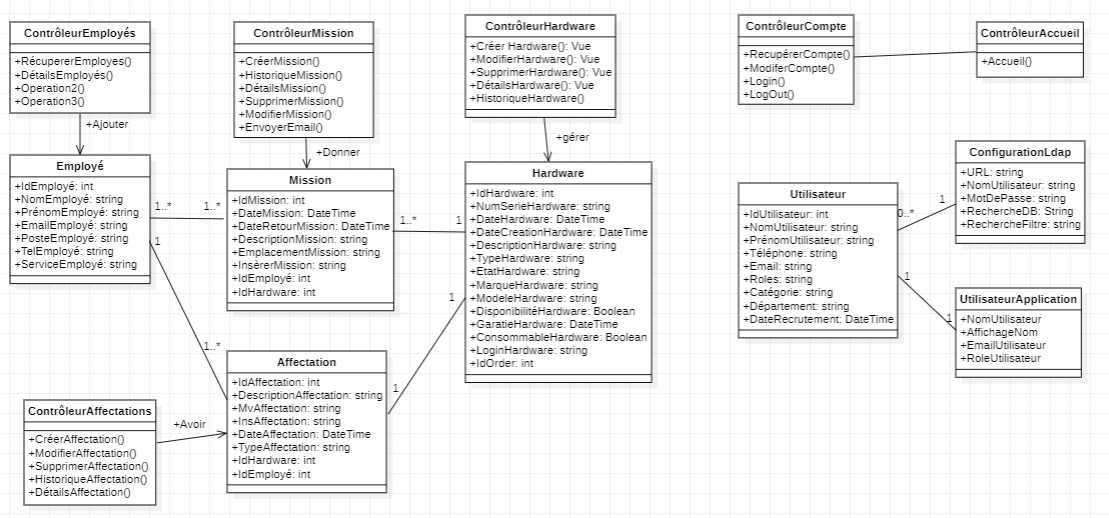
\includegraphics[width=0.9\columnwidth]{img/ClasseSprint3.png}
            \caption{Diagramme de classe Sprint (3)}
            \end{figure}
    
    \subsection{Diagramme de séquences}
        
Dans cette partie, nous étudions les diagrammes de séquences pour l'ajout d'affectation, ajout mission et l'envoie des e-mails d'alerte.

            \textbf{Diagramme de séquence "Ajout d’Affectation"}

Ce diagramme de séquence illustre les scénarios de nouvelles affectations et présente les vues dynamiques des interactions entre les objets. Il met en évidence la séquence chronologique des messages échangés entre les différents objets impliqués. 

            \begin{figure}[H]
            \centering
            
\includegraphics[width=0.9\columnwidth]{AjoutAffectation.png}
            \caption{Diagramme de séquence d'ajout Affectation d’un équipement}
            \end{figure}


            \textbf{Diagramme de séquence "Ajout Mission"}

La figure 4.24 présente le diagramme de séquence de l'Ajout Missions.

            \begin{figure}[H]
            \centering
            
\includegraphics[width=0.9\columnwidth]{AjoutMission.png}
            \caption{Diagramme de séquence d'ajout Mission d’un équipement}
            \end{figure}


            \textbf{Diagramme de séquence "envoyer un E-Mail d’alerte"}
La figure 4.25 montre le diagramme de séquence de l'email d'alerte.
            \begin{figure}[H]
            \centering
            
\includegraphics[width=0.9\columnwidth]{EnvoieMail.png}
            \caption{Diagramme de séquence envoyer un e-mail d'alerte}
            \end{figure}
            
            
        
    
    
    \subsection{Réalisation}
    
 Dans cette section, nous allons vous présenter quelques interfaces qui ont été développées lors de ce sprint.
   
   \begin{itemize}
       
   
 
    
      \item [$-$]\textbf {Ajouter une nouvelle Affectation}

        Le formulaire suivant, permet à l’utilisateur d’ajouter une nouvelle Affectation d’un équipement à un employé. \\

            \begin{figure}[H]
            \centering
            
\includegraphics[width=0.9\columnwidth]{Capture19.png}
            \caption{Ajout d’une nouvelle Affectation}
            \end{figure}

         \item [$-$]\textbf {Modifier une affectation d’un équipement}

        La figure 4.27 suivante illustre le formulaire de modification qui permettant à l’utilisateur de Modifier une affectation. \\

            \begin{figure}[H]
            \centering
            
\includegraphics[width=0.9\columnwidth]{Capture20.png}
            \caption{Modification D’une Affectation}
            \end{figure}

       \item [$-$]\textbf {Consulter la Liste des affectations}

        L’utilisateur peut consulter la liste des Affectations. A partir de cette liste, il pourra soit Modifier ou afficher les détails d’une affectation, soit supprimer une affectation ou bien faire une recherche particulière. \\

            \begin{figure}[H]
            \centering
            
\includegraphics[width=0.9\columnwidth]{Capture21.png}
            \caption{Liste de toutes les affectations}
            \end{figure}

     \item [$-$]\textbf {Afficher les Détails d’une Affectation}

        La figure 4.29 suivante montre les détails d’une affectation. A partir de cet écran l’utilisateur peut décider de : Modifier les données de cette Affectation ou de retour à la page précédente \\

            \begin{figure}[H]
            \centering
            
\includegraphics[width=0.9\columnwidth]{Capture22.png}
            \caption{Détails d’une Affectation}
            \end{figure}

         \item [$-$]\textbf {Supprimer une Affectation}

        La figure 4.30 suivante montre la page de suppression d’une affectation. A partir de cet écran l’utilisateur peut décider de : supprimer de cette Affectation ou bien de retour à la page précédente \\

            \begin{figure}[H]
            \centering
            
\includegraphics[width=0.9\columnwidth]{Capture23.png}
            \caption{La suppression d’une Affectation}
            \end{figure}

       \item [$-$]\textbf {Ajouter une mission}

        Le formulaire suivant, permet à l’utilisateur d’ajouter une nouvelle Mission \\

            \begin{figure}[H]
            \centering
            
\includegraphics[width=0.9\columnwidth]{Capture24.png}
            \caption{Ajouter une Mission}
            \end{figure}

        \item [$-$]\textbf {Modifier une mission}

        Le formulaire suivant, permet à l’utilisateur d’ajouter une nouvelle Mission \\

            \begin{figure}[H]
            \centering
            
\includegraphics[width=0.9\columnwidth]{Capture25.png}
            \caption{Modifier une Mission}
            \end{figure}

       \item [$-$]\textbf {Afficher les Détails d’une mission}

        La figure 4.33 suivante montre les détails d’une mission. A partir de cet écran l’utilisateur peut décider de : Modifier les données de cette Mission ou bien de retourné à la page précédente. \\

            \begin{figure}[H]
            \centering
            
\includegraphics[width=0.9\columnwidth]{Capture26.png}
            \caption{Détails d'une mission d'un équipement}
            \end{figure}

         \item [$-$]\textbf {Supprimer une Mission d’un équipement }

        La figure 4.34 suivante renseigne la page de suppression d’une Mission. L’utilisateur décide de supprimer de cette Mission ou bien de retourné à la page précédente \\

            \begin{figure}[H]
            \centering
            
\includegraphics[width=0.9\columnwidth]{Capture27.png}
            \caption{Suppression d'une mission }
            \end{figure}

         \item [$-$]\textbf {Consulter la liste des Mission}

        L’utilisateur peut consulter la liste des Mission. Il pourra soit Modifier ou afficher les détails, soit supprimer ou faire des rechercher \\

            \begin{figure}[H]
            \centering
            
\includegraphics[width=0.9\columnwidth]{Capture28.png}
            \caption{Liste des Missions des équipements}
            \end{figure}

         \item [$-$]\textbf {Envoyer les emails d’alertes à la fin de mission}

        Un Email de rappel sera transmis automatiquement à l’employé lorsque la date de la mission expire pour récupérer l’equipment en mission comme indiquer dans les figures 4.36 et 4.37 ci-dessous : \\

            \begin{figure}[H]
            \centering
            
\includegraphics[width=0.9\columnwidth]{EmailRappel.png}
            \caption{E-mail de rappel}
            \end{figure}

             \begin{figure}[H]
            \centering
            
\includegraphics[width=0.9\columnwidth]{ConfirmationReception.png}
            \caption{E-mail de de confirmation de la bonne réception des équipements}
            \end{figure}

        \item [$-$]\textbf {Afficher l’historique des équipements}

        Nous allons étudier dans cette partie l'historique des équipements, des mission, des bons d'achats et des fournisseurs \\

            \textbf{Historique des équipements:} \\

            L’administrateur peut consulter l’historique des équipements à partir de cette liste comme indiquer dans la figure 4.39 suivante :

            \begin{figure}[H]
            \centering
            
\includegraphics[width=0.9\columnwidth]{HistoriqueM.png}
            \caption{liste des Historiques des Matériels}
            \end{figure}

            \textbf{Historique des Missions:} \\

            L’administrateur peut consulter l’historique des Missions lister ci-dessous.

            \begin{figure}[H]
            \centering
            
\includegraphics[width=0.9\columnwidth]{HistoriqueMission.png}
            \caption{liste des Historiques des Missions}
            \end{figure}

            \textbf{Historique des Bon D’achats (Ordres) :} \\

            L’administrateur peut consulter l’historique des Bon D’achats (Ordres) à partir de cette liste.

            \begin{figure}[H]
            \centering
            
\includegraphics[width=0.9\columnwidth]{HistoriqueBA.png}
            \caption{liste des Historiques des Bons d'achat}
            \end{figure}

            \textbf{Historique des Fournisseurs:} \\

            L’administrateur peut consulter l’historique des fournisseurs à partir de cette liste.

            \begin{figure}[H]
            \centering
            
\includegraphics[width=0.9\columnwidth]{HistoriqueF.png}
            \caption{liste des Historiques des Fournisseurs}
            \end{figure}

         \item [$-$]\textbf {Envoyer à l’administrateur un E-mail d’Alerte de Stock Min}

        Les concernés vont recevoir un email d'alerte si le stock minimal est < 5 comme indiquer dans la figure 4.42 suivante  \\

            \begin{figure}[H]
            \centering
            
\includegraphics[width=0.9\columnwidth]{StockMin.png}
            \caption{E-mail d'alerte de Stock Min}
            \end{figure}

    \end{itemize}    

\subsection{Bilan de la release 2}

La release 2 représente une étape centrale du projet, car elle couvre le coeur métier de l'application : la gestion du parc informatique et le suivi des mouvements d'équipements. Elle permet de passer d'une logique de fichier statique à une logique de système d'information vivant, dans lequel chaque opération met à jour l'état du parc et enrichit l'historique.

Les apports principaux de cette release sont :

\begin{itemize}[label=\textbullet,font=\normalsize]
    \item amélioration de la visibilité sur le stock et la disponibilité des équipements ;
    \item réduction du risque de double affectation ou de perte de matériel ;
    \item meilleure traçabilité grâce à l'historique des équipements, missions, fournisseurs et commandes ;
    \item automatisation des rappels de fin de mission et des alertes de stock minimum ;
    \item mise à disposition d'un tableau de bord facilitant le pilotage opérationnel.
\end{itemize}

Cette release apporte donc une valeur métier immédiate au département IT. Elle prépare également la release suivante, qui complète le cycle de gestion par les modules liés aux commandes, fournisseurs et employés.

\section*{Conclusion}
Au cours de ce chapitre, nous avons présenté la réalisation de la deuxième Release "Gestion des équipements et Gestion des Suivis". Pour ce faire, nous avons passé par l’analyse, la conception et la réalisation des deux sprints "Gestion des équipements et Gestion des Suivis" et "Maintenance des équipements".
